%%%%%%%%%%%%%%%%%%%%%%%%%%%%%%%%%%%%%%%%%%%%%%%%%%%%%%%%%%%%%%%%%%%%%%%
% This document is based on the template: Large Colored Title Article %
%                                         Version 1.1 (25/11/12)      %
%                                                                     %
% The template was downloaded from: http://www.LaTeXTemplates.com     %
%                                                                     %
% Original author:                                                    %
% Frits Wenneker (http://www.howtotex.com)                            %
%                                                                     %
% License:                                                            %
% CC BY-NC-SA 3.0 (http://creativecommons.org/licenses/by-nc-sa/3.0/) %
%                                                                     %
% Author of this version:                                             %
% Laura M. Castro (http://www.madsgroup.org/staff/laura)              %
%                                                                     %
% Original licensing terms are maintained                             %
%%%%%%%%%%%%%%%%%%%%%%%%%%%%%%%%%%%%%%%%%%%%%%%%%%%%%%%%%%%%%%%%%%%%%%%

%----------------------------------------------------------------------------------------
%	PACKAGES AND OTHER DOCUMENT CONFIGURATIONS
%----------------------------------------------------------------------------------------

\documentclass[DIV=calc,paper=a4,fontsize=11pt,onecolumn]{scrartcl} % A4 paper and 11pt font size

\usepackage[a4paper,margin=3cm]{geometry} % 2cm margins

\usepackage[galician]{babel} % Galician language/hyphenation
\usepackage[utf8]{inputenc}
\usepackage[protrusion=true,expansion=true]{microtype} % Better typography
\usepackage{amsmath,amsfonts,amsthm} % Math packages
\usepackage[svgnames]{xcolor} % Enabling colors by their 'svgnames'
\usepackage[hang,small,labelfont=bf,up,textfont=it,up]{caption} % Custom captions under/above floats in tables or figures
\usepackage{booktabs} % Horizontal rules in tables
\usepackage{fix-cm}   % Custom font sizes - used for the initial letter in the document

\usepackage{sectsty}  % Enables custom section titles
\allsectionsfont{\usefont{OT1}{phv}{b}{n}} % Change the font of all section commands

\usepackage{fancyhdr} % Needed to define custom headers/footers
\pagestyle{fancy}     % Enables the custom headers/footers
\usepackage{lastpage} % Used to determine the number of pages in the document (for "Page X of Total")

% Headers - all currently empty
\lhead{}
\chead{}
\rhead{}

% Footers
\lfoot{\textsc{vvs-informe-prácticas}}
\cfoot{}
\rfoot{\footnotesize Páxina \thepage\ de \pageref{LastPage}} % "Page 1 of 2"

\renewcommand{\headrulewidth}{0.0pt} % No header rule
\renewcommand{\footrulewidth}{0.4pt} % Thin footer rule

\definecolor{UDC}{RGB}{206,0,124}
\definecolor{DarkUDC}{rgb}{0.75,0.75,0.75}
\definecolor{LightUDC}{RGB}{128,128,128}

\usepackage{lettrine} % Package to accentuate the first letter of the text
\newcommand{\initial}[1]{ % Defines the command and style for the first letter
\lettrine[lines=3,lhang=0.3,nindent=0em]{
\color{UDC}
{\textsf{#1}}}{}}

%----------------------------------------------------------------------------------------
%	TITLE SECTION
%----------------------------------------------------------------------------------------

\usepackage{titling} % Allows custom title configuration

\newcommand{\HorRule}{\color{UDC} \rule{\linewidth}{1pt}} % Defines the pink horizontal rule around the title

\pretitle{\vspace{-30pt} \begin{flushleft} \HorRule \fontsize{20}{20} \usefont{OT1}{phv}{b}{n} \color{DarkUDC} \selectfont} % Horizontal rule before the title

\title{INFORME DE PRÁCTICAS} % Your article title

\posttitle{\par\end{flushleft}\vskip 0.5em} % Whitespace under the title

\preauthor{\begin{flushleft}\large \lineskip 0.5em \usefont{OT1}{phv}{b}{sl} \color{DarkUDC}} % Author font configuration

\author{Repositorio de proxecto: https://github.com/andreu-barro/VVS-DFA-JAVA \\
        Participantes no proxecto: F. Javier Moure López, Emma Oitavén Carracedo, Xoan Andreu Barro Torre}

\postauthor{\footnotesize \usefont{OT1}{phv}{m}{sl} \color{Black} % Configuration for the institution name
\par\end{flushleft}\HorRule} % Horizontal rule after the title

\date{\sffamily Validación e Verificación de Software} % Add a date here if you would like one to appear underneath the title block

%----------------------------------------------------------------------------------------

\usepackage{graphicx}
\usepackage{hyperref}
\hypersetup{colorlinks=true,
            allcolors=UDC}

\usepackage{array}
\usepackage{colortbl}

%----------------------------------------------------------------------------------------

\newcommand{\hint}[1]{\begin{quote}\itshape #1 \end{quote}}

%----------------------------------------------------------------------------------------

\begin{document}

\maketitle % Print the title
\thispagestyle{fancy} % Enabling the custom headers/footers for the first page 
\clearpage

%----------------------------------------------------------------------------------------
%	ARTICLE CONTENTS
%----------------------------------------------------------------------------------------

\section{Descrición do proxecto}

Dicha aplicación simula el comportamiento de una máquina de estados

\section{Estado actual}

	Las funciones que se ocupan de la funcionalidad de nuestra aplicación son las siguientes son las que serán evaluadas:
	\begin{itemize}
		\item Clase Alphabet
		\subitem void Alphabet()
		\subitem void Alphabet(int n)
		\subitem void addNewSymbol(Symbol symbol) 
		\subitem getAlphabet : GenList<Symbol>
		\subitem getExistingObject(Symbol symbol) : Symbol
		\item Clase DFA
		\subitem DFA(GenList<State> states, Alphabet alphabet, State initialState, GenList<State> finalStates, GenList<Transition> transitions)
		\subitem getAllConnectedStates() : GenList<State>
		\subitem getConnectedDFA() : DFA
		\subitem getTransitionsTable() : String
		\item Clase State
		\subitem State(String state)
		\subitem getState() : String
		\item Clase Symbol
		\subitem Symbol(String symbol)
		\subitem getSymbol() : String
		\item Clase Transition
		\subitem void Transition(State startState, State endState, Symbol symbol)
		\subitem getEndState() : String
		\subitem getStartState() : String
		\subitem getSymbol() : Symbol
		\item Clase GenList
		\subitem void GenList()
		\subitem void GenList(int buffer)
		\subitem void add(T obj)
		\subitem void clearNulls()
		\subitem get(int n) : T
		\subitem getArray() : Object[]
		\subitem getBuffer() : int
		\subitem getExistingObject(T obj) : T
		\subitem getSize() : int
		\subitem void remove(int n)
	\end{itemize}
	
	El objetivo es probar que todas estas funciones funcionan correctamente, para ello aplicaremos pruebas de unidad, pruebas dinámicas, pruebas de rendimiento y chequearemos el estilo de programación.
	Después de aplicarle las herramientas de pruebas y utilizar las herramientas de validación como cobertura y PIT creemos que nuestras funciones son estables y que puede que tengamos una bastantes pruebas realizadas y el código testeado para fiarnos de él. 

\subsection{Compoñentes avaliados}

Si ejecutamos \textit{mvn test org.pitest:pitest-maven:mutationCoverage site} en la raiz del proyecto se generarán reports sobre los tests. \\

Los genera en target/site/Index.html, ahí navegamos a project reports. \\

\section{Especificación de probas}

\subsection{Pruebas de unidad}
\href{Informes/documentoUnidad.txt}{Pruebas de unidad} \\

\subsection{Pruebas basadas en propiedades}
\href{Informes/documentoPropiedades.txt}{Pruebas basadas en propiedades} \\

\subsection{Validación de calidad de las pruebas}
\href{http://cobertura.sourceforge.net/}{Cobertura})
\href{http://pitest.org/}{Mutation Testing: PIT})

\subsection{Pruebas dinámicas de unidad}
\href{Informes/documentoDinamicasUnidad.txt}{Pruebas dinámicas de unidad} \\

\subsection{Pruebas no funcionales}
Hemos probado todas los métodos de todos las clases que tenemos (Alphabet, DFA, GenList, State, Symbol y Transition) \\

Nos hemos ayudado de JETM y el modelo que hemos utilizado es este: 
\href{Informes/documentoRendimiento.txt}{Pruebas no funcionales} \\

\subsection{Pruebas estructurales}
\href{http://checkstyle.sourceforge.net/}{CheckStyle})

	\section{Registro de pruebas}
	\subsection{Pruebas unidad: JUnit}
	JUnit se utiliza para realizar pruebas unitarias sobre nuestra aplicación, nos sirven para encontrar errores y solventar los problemas en la programación de forma manual.
	Se realizan pruebas de todas las funciones implementadas en la aplicación.
	Los casos de prueba se implementan manualmente como parte de funciones de prueba, utilizamos la directiva assertEqual(Expected, Expr).
	\subsection{Pruebas basadas en propiedades: Quickcheck}
	QuickCheck es una  herramienta para generar automáticamente y ejecutar casos de prueba aleatorios, basados en especificaciones de propiedades. Es decir, ejecutar pruebas con esta herramienta, significa instanciar las propiedades n veces. Las pruebas se detienen al encontrar un caso concreto en el que la propiedad no se cumple
	(contraejemplo).La ejecución con éxito significa que ninguno de los casos generados incumplió la propiedad
	Se crean generadores de:
	\begin{itemize}
		\item GeneradorAlphabet
		\item GeneradorDFA
		\item GeneradorState
		\item GeneradorSymbol
		\item GeneradorTransition
		\item GeneradorGenList
	\end{itemize}
	
	La programación de generadores para aplicar Quickcheck se realiza en el siguiente paquete: es.udc.fic.vvs.vvsproject.generadorTest
	
	\subsection{Validación de calidad de las pruebas: Cobertura}
	Cobertura( \href{http://cobertura.sourceforge.net/}{Plugin cobertura}) es una herramienta libre (GPL) escrita en Java, que nos permite comprobar el porcentaje de código al que accedemos desde los test. Es decir, Cobertura nos permite saber cuanto código estamos realmente probando con nuestros test.
	De esta forma Cobertura se convierte en una potente herramienta de trabajo, ya que lo podemos usar como medida de calidad (mientras más código tengamos probado, más garantías tenemos de que podemos hacer refactorizaciones sin peligro).
	Nuestro objetivo es llegar a cobertura cercana a 100.
	
	\subsection{Pruebas dinámicas de unidad: Mockito}
	Para poder crear un buen conjunto de pruebas unitarias, es necasario que nos centremos exclusivamente en la clase a testear, simulando el funcionamiento de las capas inferiores (pensad por ejemplo en olvidarnos de la capa de acceso a datos, DAO). De esta manera estaremos creando test unitarios potentes que os permitiría detectar y solucionar los errores que tengáis o que se cometan durante el futuro del desarrollo de vuestra aplicación.
	Para esta tarea nos apoyaremos en el uso de mock objects, que no son más que objetos que simulan parte del comportamiento de una clase, y más especificamente vamos a ver una herramienta que permite generar mock objects dinámicos, mockito. \\
	
	Pruebas que se realizarán en el paquete es.udc.vvs.dfa.mockito, sólo se realizarán las pruebas del servidor, debido a que las pruebas de componentes ya son pruebas de unidad.
	\subsection{Pruebas no funcionales: JETM}
	JETM permite realizar pruebas de rendimiento y comprobar la velocidad de ejecuciones al implementar unas pruebas con n iteraciones. Se pueden generar test con múltiples iteraciones para detectar problemas de rendimiento. \\
	
	Pruebas que se realizarán en el paquete es.udc.vvs.dfa.rendimiento
	\subsection{Validación de calidad de las pruebas (mutación testing): PIT}
	
	El  método que utilizaban en el sistema para realizar estas mediciones lo denominaba “Programa mutado”.
	Básicamente, el Mutation testing consiste en introducir pequeñas modificaciones en el código fuente de la aplicación, a las que denominaremos mutaciones o mutantes.
	
	Si las pruebas pasan al ejecutarse sobre el mutante, el mutante sobrevive.
	Si las pruebas no pasan al ejecutarse sobre el mutante, el mutante muere
	El objetivo es que todos los mutantes mueran, así podremos decir que el test responde a la definición concreta del código y que lo prueba correctamente.
	Este concepto se basa en dos hipótesis:
	\begin{itemize}
		\item Hipótesis del programador competente: La mayoría de los errores introducidos por programadores Senior consisten en pequeños errores sintácticos.
		\item Hipótesis del efecto de acoplamiento: Pequeños fallos acoplados pueden dar lugar a otros problemas mayores.
	\end{itemize}
	Problemas de mayor orden serán revelados por mutantes de mayor orden, que se crean mediante la unión de multiples mutaciones.
	
	\subsection{Pruebas estructurales: CheckStyle}
	
	Checkstyle es una herramienta de desarrollo que ayudar a los programadores a escribir código Java para que se adhiera a un estándar de codificación. Automatiza el proceso de comprobación de código Java. Esto lo hace ideal para los proyectos a los que se desea aplicar un estándar de codificación.
	
	Checkstyle es altamente configurable y se puede hacer para apoyar casi cualquier estándar de codificación. De tal manera que se puedan suministrar diferentes estándares de código para su posterior comprobación mediante la herramienta.
	
	Reglas del CheckStyle
	El conjunto de reglas disponible es muy completo y está clasificado en los siguientes grupos:
	\begin{itemize}
		\item Comentarios Javadoc: facilitar el mantenimiento pasa por comentar el código, pero luego los comentarios también hay que mantenerlos... CheckStyle tiene muchas reglas para los javadoc y es muy flexible. Te permite, por ejemplo, obligar a comentar los nombres de clases, todos los métodos menos los get/set y los atributos públicos.
		\item Convenciones de nombres: puedes definir una expresión regular para el nombre de todo. 
		\item 	Cabeceras: expresiones regulares para la cabecera de los ficheros.
		\item Imports: reglas para los import, como no usar *, imports sin usar, etc.
		\item Violaciones de tamaño: define un máximo para el tamaño de tus clases, métodos, líneas y número de parámetros de un método.
		Espacios en blanco: un montón de reglas para definir donde se ponen espacios en blanco y tabuladores en el código.
		\item Modificadores: establece un orden para los modificadores y evita modificadores innecesarios.
		\item Bloques: reglas para los bloques de código y sus llaves.
		\item Problemas en la codificación: Acá hay de todo, desde malas prácticas tipo asignaciones internas y posibles fuentes de bugs como definir un método equals que no es el equals(Object), a cosas más estéticas o poco prolijas, como que el default sea el último elemento en un switch o paréntesis innecesarios.
		\item Diseño de clases: varias reglas sobre el diseño de interfaces y clases, con especial atención en las excepciones.
		\item Duplicados: te permite definir un mínimo de líneas para buscar código duplicado en tus clases.
		\item Métricas: define máximos para métricas como complejidad ciclomática, complejidad de expresiones lógicas, npath, líneas de código seguidas sin comentar y dependencia de clases.
		\item Misceláneo: variables final, indentación, un buscador de expresiones regulares y varias cosas más.
		\item J2EE: reglas para EJBs.
		\item Otros: internos a CheckStyle y activados por defecto.
		\item Filtros: para eventos de auditoria del propio CheckStyle, no hace falta mirarlos.
	\end{itemize}	
	Checkstyle es una herramienta de desarrollo para ayudar a los programadores escribir código Java que se adhiere a un estándar de codificación. 
	Para comprobar el estilo, pasamos la herramienta CheckStyle a nuestra aplicación y comprobamos el resultado:
	
	
	\section{Registro de errores}
	\subsection{Pruebas unidad: JUnit}
	Se puede comprobar que no fallan.
	
	\subsection{Pruebas dinámicas de unidad: Mockito}
	Se puede comprobar que no fallan.
	
	\subsection{Validación de la calidad de las pruebas: Cobertura}
	
	Estado inicial:
	
	
		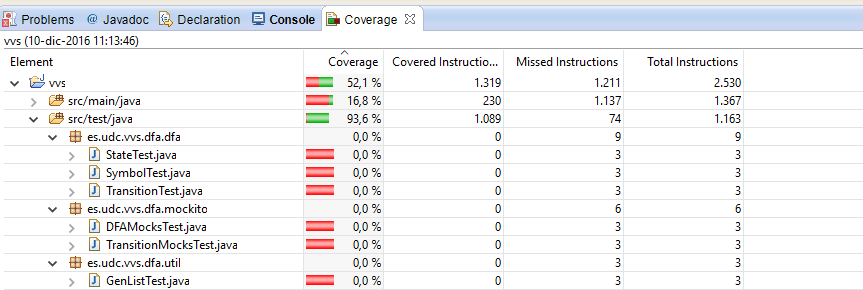
\includegraphics[width=15cm]{Imagenes/sinCobertura.png}
	
	
	Estado final:
	--
	
		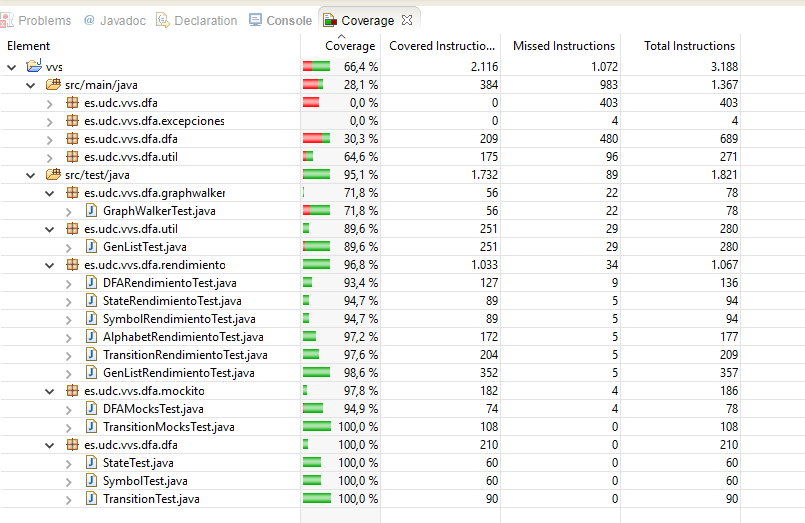
\includegraphics[width=15cm]{Imagenes/Cobertura.png}
	
	\subsection{Pruebas no funcionales: JETM}
	Resultado del rendimiento de JETM:
	\href{Informes/SiteTestInicial/jetm-timing-report.html}{Informe JETM} \\
	
	%	\includegraphics[width=16cm]{Imagenes/JETM1.png} \\
	%	\includegraphics[width=16cm]{Imagenes/JETM2.png} \\
	Con JETM hemos tenido problemas  a la hora de que nos genera el site todos los resultados de las pruebas. Sí genera los resultados guardandolos en un xml con todos los resultados, pero no los muestra en la página de resultados del site.
	\subsection{Validación de calidad de las pruebas (mutación testing): PIT}
	Realizado el mutation testing, resultados:
	
	\href{Informes/pit-reports/index.html}{Informe PIT} \\
	
	\subsection{Pruebas estructurales: CheckStyle}
%	Podemos comprobar los errores encontrados en el siguiente informe: \href{Informes/SiteTestInicial/checkstyle.html}{Informe CheckStyle} \\
	Al pasar la herramienta de CheckStyle descubrimos que nuestra aplicación tiene muchos errores de estilo, es decir, que no cumple el estándar de programación java.
	
	Resumen de errores encontrados:
	\begin{itemize}
		\item Faltan comentarios: En la mayoría de clases faltan comentarios javadoc. Se añaden.
		\item Mala indexación código y espacios: Se reestructura el código para que solventar dichos errores.
	\end{itemize}
	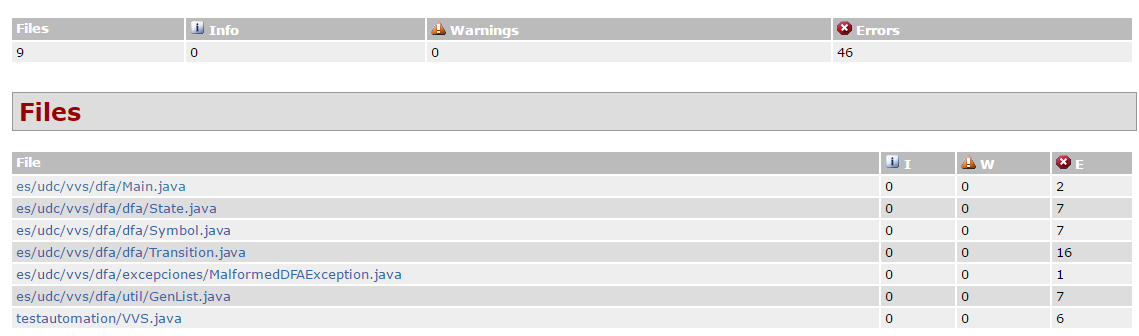
\includegraphics[width=15cm]{Imagenes/erroresCheckStyle.png} \\
	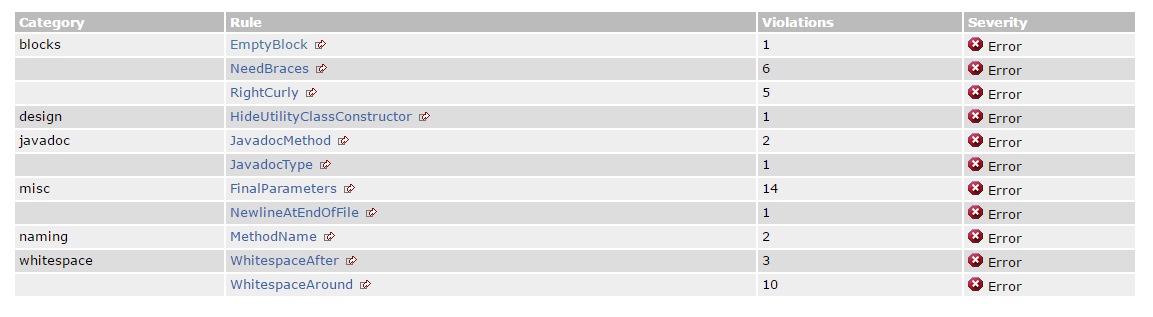
\includegraphics[width=15cm]{Imagenes/checkStyleErrores.png} \\
	Después de revisar los errores encontrados, resolvemos los errores de estilo encontrados y este es el resultado:
	  \href{Informes/checkStyle-report/checkstyle.html}{Informe CheckStyle} \\

	%		\includegraphics[width=15cm]{Imagenes/CheckStyleResut.png} \\
	\subsection{Pruebas estáticas/estructurales: FindBugs}
	
	FindBugs es un programa que utiliza el análisis estático para buscar errores en el código de Java.
	
	\href{Informes/findBugs-report/findbugs.html}{Informe Find bugs} \\
	
	Errores encontrados inicialmente:
	
	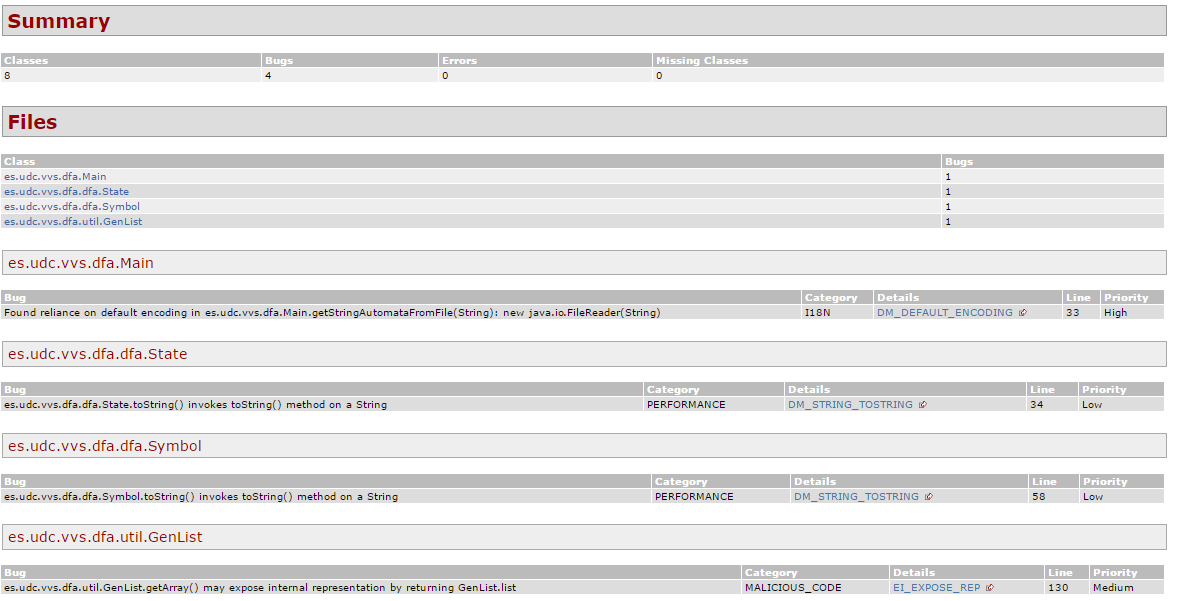
\includegraphics[width=15cm]{Imagenes/findBugs1.png} \\
	
	Después de identificar los errores, resolvedos los problemas mencionados y comprobamos el resultado:\\
	
	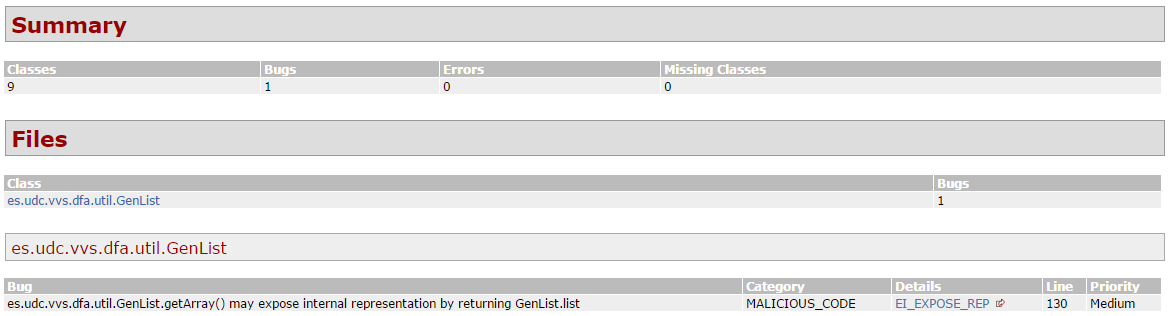
\includegraphics[width=15cm]{Imagenes/findBugs2.png} \\

\section{Estatísticas}

\hint{Deben incluírse como mínimo:
  \begin{itemize}
    \item Número de erros encontrados diariamente e semanalmente.
    \item Nivel de progreso na execución das probas.
    \item Análise do perfil de detección de erros (lugares, compoñentes, tipoloxía).
    \item Informe de erros abertos e pechados por nivel de criticidade.
    \item Avaliación global do estado de calidade e estabilidade actuais.
  \end{itemize}}

\section{Outros aspectos de interese}

\hint{Neste apartado se incluirán todos aqueles aspectos e detalles que non se
  mencionaran nos puntos anteriores, pero que o equipo do proxecto considere que
  poden aportar valor.}

\end{document}
